
\documentclass{report}
\usepackage[a4paper,top=0px,bottom=50px]{geometry}

\usepackage[english]{babel}
\usepackage[utf8]{inputenc}
\usepackage[T1]{fontenc}

\usepackage{adjustbox}
\usepackage{caption}
\usepackage{subfigure}
\usepackage{ragged2e}
\usepackage{float}
\usepackage{minitoc}
\usepackage{hyperref}
\usepackage{graphicx}
\usepackage{pifont}
\usepackage{wrapfig,lipsum}
\usepackage{setspace}  % Double spacing
\renewcommand{\thesection}{\Roman{section}} 


\begin{document}


\chapter{Project Context}

\textbf{\Large Introduction}
\vspace{30px}
\textnormal{
\\In our first chapter, we will focus on presenting the general context surrounding our project. We will first start by presenting our host organization, then we'll proceed with explaining the existing situation in which the spotlight will be put on the current problems and critiques that will be a main factor to form the solutions that will, later on, be elaborated.}

\section{Host Organization}
\subsection{Host organization presentation}
\textnormal{
OptimaSoft is a software engineering company founded in 2006 with the goal of meeting the needs of small and medium companies in terms of IT ressource management and adaptation to new technologies. It sets as its first objective contributing to the efficiency and success of its customers  the reliability of its information systems and covers various sectors and activities.
}
\subsection{Activity Sectors}
\textnormal{
OptimaSoft acts in the following sectors : 
}
\begin{itemize}
\item [\ding{51}]  Hospitality and Tourism
\item  [\ding{51}]Travel Agencies
\item [\ding{51}]Services
\item [\ding{51}]Wholesale trade
\item [\ding{51}]Export Trade
\item [\ding{51}]Textiles and Industries
\item [\ding{51}]Catering and Entertainment Area
\item [\ding{51}]Firm of expertise and bookkeeping 
\item[\ding{51}] Real Estate development
\end{itemize}

\section{General Project Presentation}
 \subsection{Context Presentation}
\textnormal{
Room booking and characteristics specification has always been the fundamental parts of hotel reservation. In our case our web app allows users to fulfill these steps online and provide offers and recommendations in case they decide to become a client. It also makes managing hotel data easier than ever by providing the admin with graphic visualizations for hotel statistics in the admin dashboard. Our app aims to provide comfort to both users and admins.  
}

 \subsection{Problem Definition}
\textnormal{
 During certain times of the year, making hotel reservations could be a tough task as hotel lobbies be full of customers potentially waiting for hours to confirm a reservation. In addition regular clients tend to get no special treatment than one in a time customers. And finally, as hotel data can be a ton to manage, it is sometimes a harder than it should be task for admins to understand what exactly is going on in the hotel they're trying to manage and therefore struggle to make the right decisions.
}

\section{Methodological Choice}
\textnormal{
An analysis and conception method is a process that aims to formalize the preliminary stages of the development of a system to make the development more faithful to the customer needs.
There are many methods from which we can mention the Unified Process (UP), Y Method and Agile Approaches.
In the case of our project we chose to work with the agile approach for reasons between which we can mention our familiarity with it. 
}

 \subsection{Agile Approaches}
\textnormal{
Agile approaches, first being invented in 1913, dedicated to upgrade the process of analysis and conception and reduce the failure rate. They also assure a superior value  product, client satisfaction and the prediction and planning of costs. 
Agile approaches rely on cycles of iterative, incremental and adaptive development. 
From the agile approaches out there we can mention : 
}

 \begin{itemize}
\item [\ding{51}]  Scrum
\item  [\ding{51}]Extreme Programming (XP) 
\item [\ding{51}]Rapid Application Development (RAD)

\end{itemize}

\subsection {SCRUM Methodology}
\textnormal{
Scrum is an agile development methodology used in the development of software based on iterative and incremental processes. It's adaptable, fast, flexible and effective agile framework that is designed to deliver value to the customer throughout the development of the project. The primary objective of scrum is to satisfy the customer's need through an environment of transparency in communication, collective responsibility and continuous progress. The development starts from a general idea of what needs to be built, elaborating a list of characteristics ordered by priority.
}

\begin{center}
 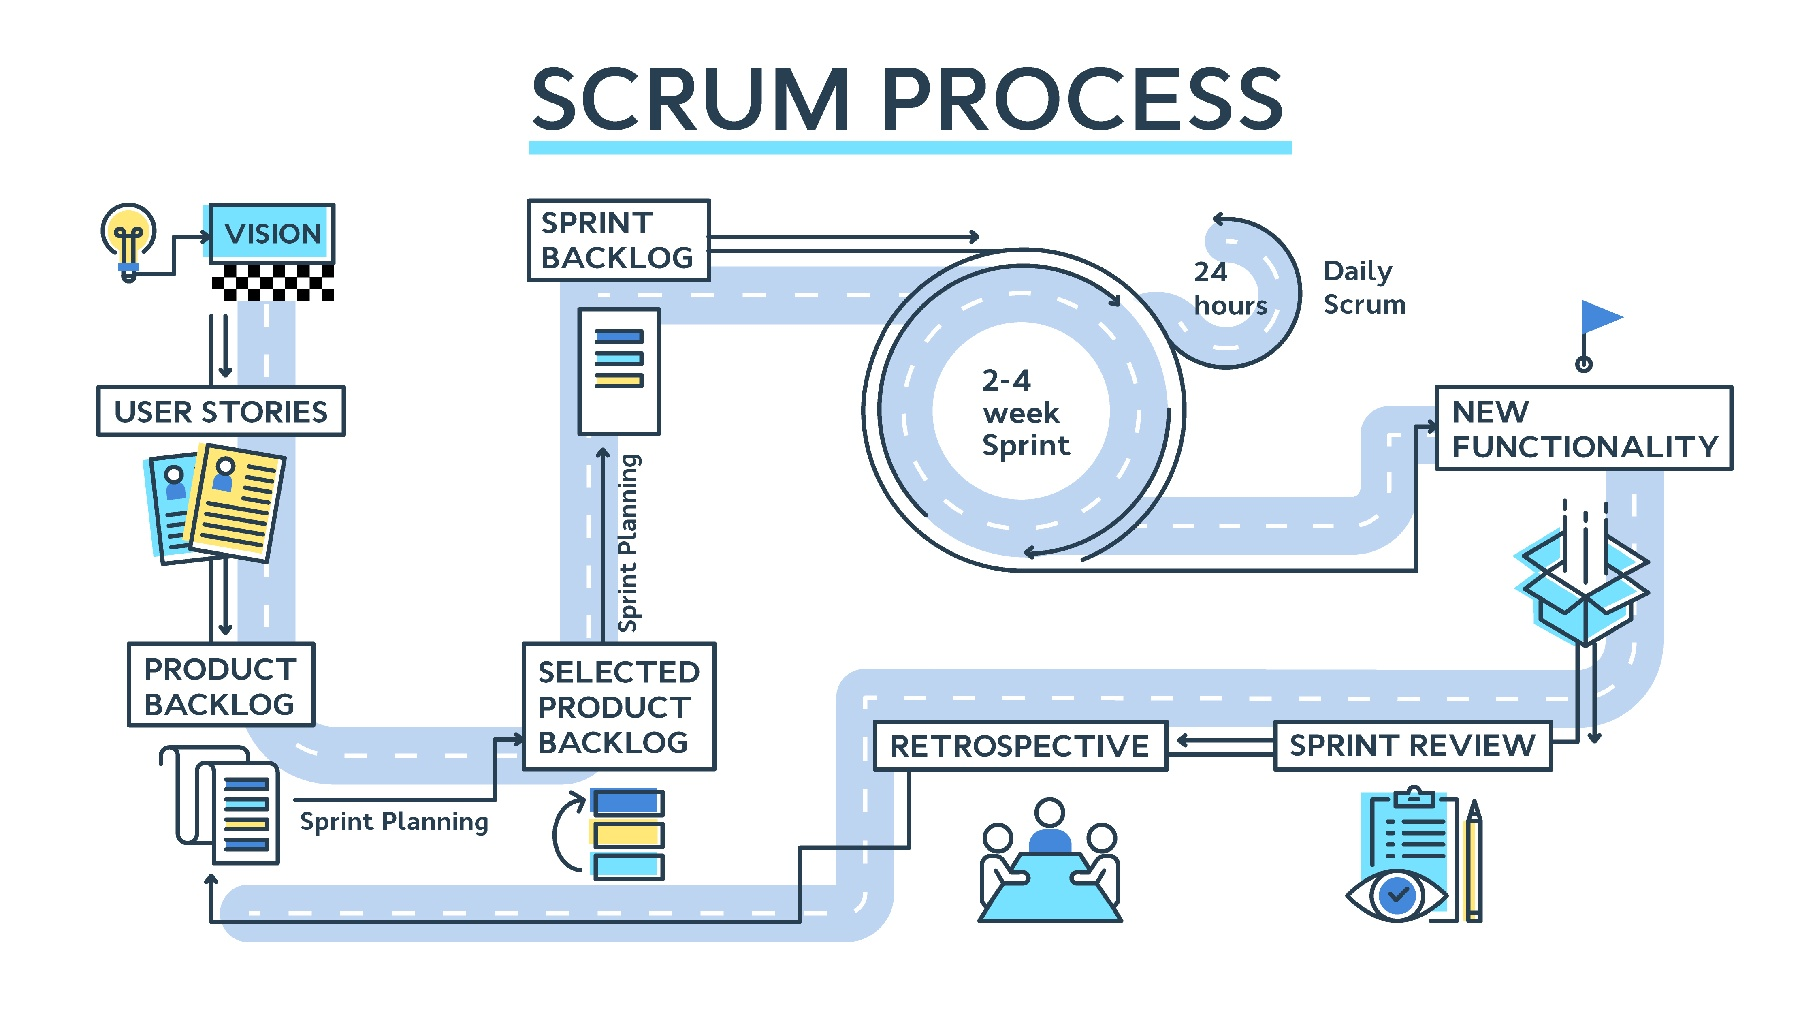
\includegraphics[scale=0.2]{images/Scrum.jpg}
\end{center}
\captionof{figure}{Scrum Process}

\subsection {Scrum Project Roles}

\textnormal{
In a Scrum project,there are three core roles:
}
\begin{itemize}
    \item[--]\textbf{\normalsize Product Owner :} \textnormal{The product owner represents stakeholders, who are typically customers. To ensure the scrum team is always delivering value to stakeholders and the business, the product owner determines product expectations, records changes to the product and administers a scrum backlog, a detailed and constantly updated to-do list for the scrum project. The product owner is also responsible for prioritizing goals for each sprint, based on their value to stakeholders, such that the most important and deliverable features are built in each iteration.}
\end{itemize}

\begin{itemize}
    \item[--]\textbf{\normalsize Scrum Master :} \textnormal{The scrum master is the facilitator of the scrum development process. In addition to holding daily meetings with the scrum team, the scrum master makes certain that scrum rules are being enforced and applied as intended. The scrum master’s responsibilities also include coaching and motivating the team, removing impediments to sprints, and ensuring that the team has the best possible conditions to meet its goals and produce deliverable products.}
\end{itemize}

\begin{itemize}
    \item[--]\textbf{\normalsize Scrum Team / Developers :} \textnormal{The scrum team is a self-organized group of three to nine individuals who have the business, design, analytical and development skills to carry out the actual work, solve problems and produce deliverable products. Members of the scrum team self-administer tasks and are jointly responsible for meeting each sprint’s goals.}
\end{itemize}
\begin{center}
 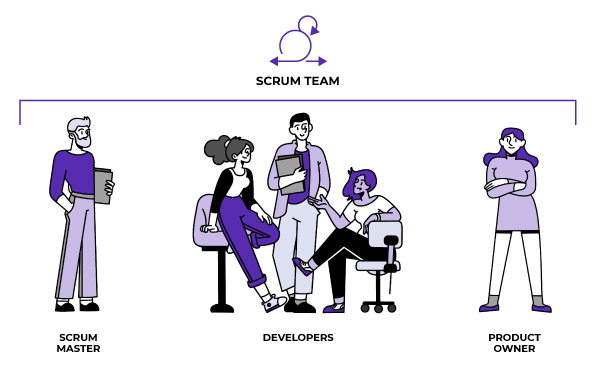
\includegraphics[scale=0.4]{images/roles.jpg}
\end{center}
\captionof{figure}{Scrum Roles}

\subsection {Modeling Language}
 \textnormal{
For our project, we chose to use UML as a modeling language.\newline
UML, short for Unified Modeling Language, is a standardized modeling language consisting of an integrated set of diagrams, developed to help system and software developers for specifying, visualizing, constructing, and documenting the artifacts of software systems, as well as for business modeling and other non-software systems. The UML represents a collection of best engineering practices that have proven successful in the modeling of large and complex systems. The UML is a very important part of developing object oriented software and the software development process. 
}
\begin{center}
 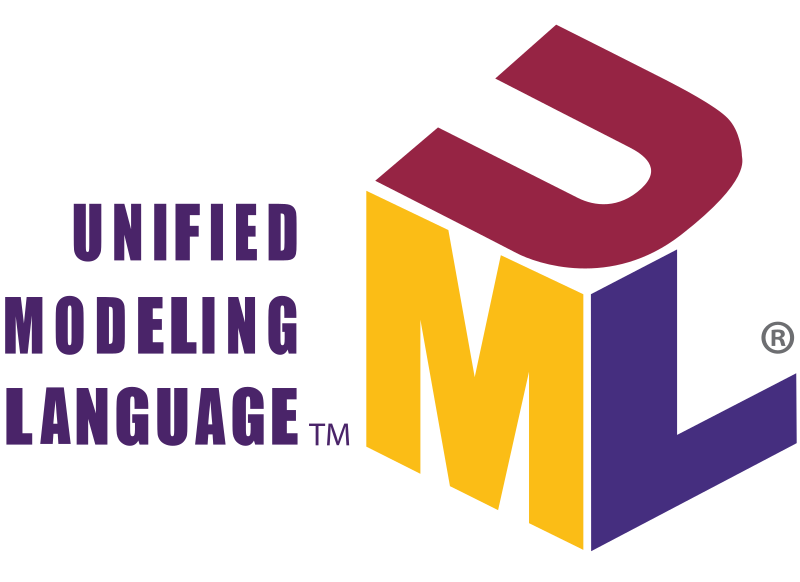
\includegraphics[scale=0.15]{images/uml.png}
\end{center}
\captionof{figure}{UML Logo}
\end{document}
